%presentation.tex
%Andy Sayler
%Constantin Berzan
%-----------------------------------------------------------------------------%
\documentclass[xcolor=dvipsnames]{beamer}
%\useoutertheme{default}
%\usetheme{Boadilla}
\setbeamercovered{transparent=25}
\setbeamertemplate{blocks}[rounded][shadow=false] 
\setbeamertemplate{navigation symbols}{}
\usepackage{graphics}

\title[SLAM]{More SLAM}
%\subtitle[]{}
\author[ C. Berzan \& A. Sayler]{ Constantin Berzan \& Andy Sayler}
\institute[Tufts University]{
  Tufts University\\
  COMP150 - BBR\\
  \texttt{constantin.berzan@tufts.edu}\\
  \texttt{andrew.sayler@tufts.edu}
}
\date[Dec. 14, 2010]{Tuesday, December 14\textsuperscript{th}, 2010}

\begin{document}
  
  %----Title Slide------------------------------------------------------------%
  \begin{frame}[plain]
    \titlepage
  \end{frame}
  
  \section*{Outline}  
  %----Outline Slide----------------------------------------------------------%
  \begin{frame}{Outline}
    \pause
    \tableofcontents[pausesections]
  \end{frame}
  
  \section{Overview}
  %----SLAM Overview - Andy--------------------------------------------------%
  \begin{frame}{SLAM Overview}
    
  \end{frame}
  
  \section{Landmarks}
  %----Landmarks - Constantin--------------------------------------------------%
  \begin{frame}{Landmark extraction}
    Landmarks: easily reobservable features in the environment, used in
    localization
    \vspace{1cm}

    Our landmark extraction algorithm:
    \begin{itemize}
    \item Extract lines from laser readings (RANSAC)
    \item Determine the origin of the world coordinate system using the
          estimated robot position
    \item Project origin onto each line, take resulting points as landmarks
    \end{itemize}
  \end{frame}

  \begin{frame}{Line extraction}
    RANSAC: Random Sample Consensus
    \vspace{0.5cm}

    Input: set of points $\mathcal{P}$

    Output: set of fitted lines $\mathcal{L}$

    Algorithm:
    \begin{itemize}
    \item Select random subset of points $\mathcal{P}_{sample}$
    \item Fit line $\ell_{sample}$ through sample points
    \item Compute set $\mathcal{P}_{consensus}$ of all points in $\mathcal{P}$
          that are within a small distance of the line $\ell_{sample}$
    \item If there are enough such points, fit a new line
          $\ell_{consensus}$ through $\mathcal{P}_{consensus}$.
          Add $\ell_{consensus}$ to the output set $\mathcal{L}$, and
          remove all fitted points $\mathcal{P}_{consensus}$ from $\mathcal{P}$
    \item Repeat until all points are fitted, or a maximum number of iterations
          is reached
    \end{itemize}
  \end{frame}

  {
  \usebackgroundtemplate{\includegraphics[width=\paperwidth]{ransac-mix.png}}
  \begin{frame}{Line extraction example}
  \end{frame}
  }

  {
  \usebackgroundtemplate{\includegraphics[width=\paperwidth]{landmark-mix.png}}
  \begin{frame}{Landmark extraction example}
  \end{frame}
  }

  \section{EKF}
  %----EKF - Andy--------------------------------------------------%
  \begin{frame}{EKF}
    
  \end{frame}
  
  \section{Demo}
  %----Demo - Both--------------------------------------------------%
  \begin{frame}{Demo}
    
  \end{frame}
  

\end{document}
